
\section{Utilización de la herramienta de captura}

Para realizar la captura de paquetes, se implementó una herramienta en python. Para poder utilizar la misma se debe tener instalados los siguientes paquetes:

\begin{itemize}
	\item python 2.7
	\item pyqt4 (para python 2.7)
	\item scapy
\end{itemize}

Para ejecutar la aplicación se debe ejecutar el siguiente comando en consola:

\begin{figure}[h!]
	\centering
	\begin{lstlisting}
	[ignacio@desktop ~]$ sudo ./arp
	\end{lstlisting}
\end{figure}

ó:


\begin{figure}[h!]
	\centering
	\begin{lstlisting}
	[ignacio@desktop ~]$ sudo python2 arp
	\end{lstlisting}
\end{figure}

El archivo \emph{arp} se encuentra dentro de la carpeta que contiene la herramienta.

\begin{figure}[h!]
	\caption{Herramienta de Captura, pantalla principal.}
	\centering
	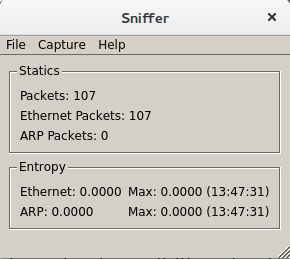
\includegraphics[width=0.25\textwidth]{graficos/tool/tool}
\end{figure}

Para comenzar una nueva captura, se debe elegir la opción \emph{Start} del menú \emph{Capture}. Para detener la misma seleccionar la opción \emph{Stop} del mismo menú.

% mostrar menú (no le puedo sacar una foto... WTF?!)

También la aplicación da la opción de realizar capturas por intervalos de tiempo en minutos. Para activarla, seleccionar \emph{Interval} del menú \emph{Capture}.

\begin{figure}[h!]
        \centering
        \begin{subfigure}[b]{0.3\textwidth}
                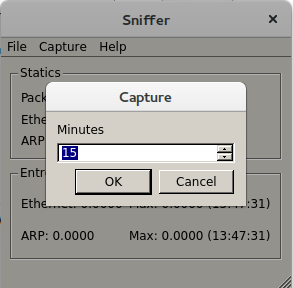
\includegraphics[width=\textwidth]{graficos/tool/tool_interval}
                \caption{Duración de la captura}
        \end{subfigure}%
        ~ %add desired spacing between images, e. g. ~, \quad, \qquad, \hfill etc.
          %(or a blank line to force the subfigure onto a new line)
        \begin{subfigure}[b]{0.3\textwidth}
                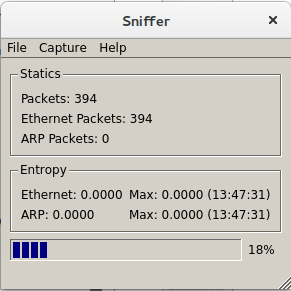
\includegraphics[width=\textwidth]{graficos/tool/tool_progress}
                \caption{Evolución de la captura}
        \end{subfigure}
        ~ %add desired spacing between images, e. g. ~, \quad, \qquad, \hfill etc.
          %(or a blank line to force the subfigure onto a new line)
        \begin{subfigure}[b]{0.3\textwidth}
                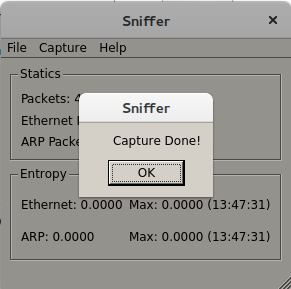
\includegraphics[width=\textwidth]{graficos/tool/tool_done}
                \caption{Captura terminada}
        \end{subfigure}
        \caption{Capturando durante un intervalo de tiempo en minutos.}\label{fig:interval}
\end{figure}

Para almacenar la información capturada por la herramienta, la misma posee dos opciones bajo el menú \emph{File}. Dichas opciones son:

\begin{description}
	\item[Save Capture]	Guarda los paquetes capturados dentro de un archivo de texto plano.
	\item[Save Entropy] A cada segundo la herramienta calcula la entropía de ambas fuentes. Esta opción salva dicha información en un archivo de texto plano.
\end{description}

